\documentclass[twocolumn]{article}

% Gói ngôn ngữ và font chữ
\usepackage[utf8]{inputenc}
\usepackage[T5]{fontenc}
\usepackage[vietnamese]{babel}

% Gói toán học
\usepackage{amsmath}
\usepackage{amssymb}
\usepackage{amsfonts}

% Gói hình ảnh và bảng
\usepackage{graphicx}
\usepackage{booktabs} % Cho bảng đẹp hơn
\usepackage{tabularx}
\usepackage{multirow}
\usepackage{caption}
\usepackage{subcaption}
\usepackage{adjustbox}
\usepackage{lscape}
\usepackage{rotating}
\usepackage{stfloats} % Để xử lý vị trí float 2 cột

% Gói layout và siêu liên kết
\usepackage{geometry}
\usepackage{url}
\usepackage[hidelinks]{hyperref}

% Thiết lập layout trang
\geometry{
 a4paper,
 total={170mm,257mm},
 left=20mm,
 top=20mm,
}
\setlength{\columnsep}{6mm}

% Thông tin tác giả và tiêu đề
\title{\textbf{SVIP: Semantically Contextualized Visual Patches for Zero-Shot Learning}}
\author{
    Zhi Chen$^{1*}$, Zecheng Zhao$^{2*}$, Jingcai Guo$^3$, Jingjing Li$^1$, Zi Huang$^2$ \\
    \small $^1$University of Southern Queensland, $^2$University of Queensland \\
    \small $^3$The Hong Kong Polytechnic University \\
    \small $^4$University of Electronic Science and Technology of China \\
    \small \texttt{uqzhichen@gmail.com, helen.huang@uq.edu.au}
}
\date{July 10, 2025}


\begin{document}

\maketitle
\def\thefootnote{*}\footnotetext{Đóng góp ngang nhau. Công việc được thực hiện khi còn ở Đại học Queensland.}\def\thefootnote{\arabic{footnote}}

\begin{abstract}
Zero-shot learning (ZSL) nhằm mục đích nhận dạng các lớp chưa từng thấy mà không có các mẫu huấn luyện được gán nhãn bằng cách tận dụng các bộ mô tả ngữ nghĩa cấp lớp như các thuộc tính. Một thách thức cơ bản trong ZSL là sự sai lệch ngữ nghĩa (semantic misalignment), trong đó thông tin không liên quan đến ngữ nghĩa có trong các đặc trưng thị giác gây ra sự mơ hồ cho tương tác thị giác-ngữ nghĩa. Không giống như các phương pháp hiện có giúp triệt tiêu thông tin không liên quan đến ngữ nghĩa sau xử lý (post hoc) trong không gian đặc trưng hoặc không gian mô hình, chúng tôi đề xuất giải quyết vấn đề này ở giai đoạn đầu vào, ngăn chặn các bản vá không liên quan đến ngữ nghĩa lan truyền qua mạng. Để đạt được mục tiêu này, chúng tôi giới thiệu Semantically Contextualized Visual Patches (SVIP) cho ZSL, một framework dựa trên transformer được thiết kế để tăng cường sự liên kết thị giác-ngữ nghĩa. Cụ thể, chúng tôi đề xuất một cơ chế lựa chọn bản vá tự giám sát (self-supervised) để học cách xác định các bản vá không liên quan đến ngữ nghĩa trong không gian đầu vào một cách ưu tiên. Cơ chế này được huấn luyện với sự giám sát từ các điểm chú ý được tổng hợp trên tất cả các lớp transformer, ước tính điểm ngữ nghĩa của mỗi bản vá. Vì việc loại bỏ các bản vá không liên quan đến ngữ nghĩa khỏi chuỗi đầu vào có thể làm phá vỡ cấu trúc đối tượng, chúng tôi thay thế chúng bằng các nhúng bản vá có thể học được (learnable patch embeddings). Với việc khởi tạo từ các nhúng từ (word embeddings), chúng tôi có thể đảm bảo chúng vẫn có ý nghĩa ngữ nghĩa trong suốt quá trình trích xuất đặc trưng. Các thí nghiệm sâu rộng trên các bộ dữ liệu ZSL tiêu chuẩn đã chứng minh rằng SVIP đạt được kết quả hiệu suất hiện đại (state-of-the-art) đồng thời cung cấp các biểu diễn đặc trưng có khả năng diễn giải tốt hơn và giàu ngữ nghĩa hơn. Mã nguồn có sẵn tại \url{https://github.com/uqzhichen/SVIP}.
\end{abstract}


\section{Giới thiệu}

Zero-shot learning (ZSL) \cite{28, 37, 58} là một mô hình học tập cơ bản trong thị giác máy tính cho phép các mô hình nhận dạng các lớp chưa từng thấy trong quá trình huấn luyện. Các phương pháp ZSL thường chuyển đổi việc phân loại thành một nhiệm vụ hồi quy, trong đó các bộ mô tả ngữ nghĩa cấp lớp, chẳng hạn như các thuộc tính \cite{21} đóng vai trò là các nhãn mềm. Ví dụ, mỗi chiều của một véc-tơ thuộc tính có thể chỉ ra sự hiện diện hoặc vắng mặt của một khái niệm như màu hồng. Tại thời điểm kiểm tra, véc-tơ thuộc tính được dự đoán sẽ được so sánh với các thuộc tính của các lớp chưa từng thấy, và lớp tương tự nhất sẽ được chọn.

Sự sai lệch ngữ nghĩa (Semantic misalignment) là một thách thức cơ bản trong ZSL \cite{1, 4, 9, 27, 30, 46}. Hình ảnh thô thường chứa các chi tiết không liên quan đến ngữ nghĩa không được mô tả bởi các thuộc tính. Ví dụ, sự lộn xộn của nền, các biến thể ánh sáng, hoặc các đối tượng xung quanh có thể tạo ra các mẫu gây hiểu lầm. Do đó, mô hình có thể tập trung vào các đặc trưng không quan trọng thay vì các tín hiệu ngữ nghĩa có liên quan. Vì các chi tiết ngoại lai này không được chú thích rõ ràng trong các véc-tơ thuộc tính, chúng phá vỡ sự liên kết thị giác-ngữ nghĩa bằng cách làm loãng các thuộc tính chính như màu sắc và hình dạng. Điều này làm cho mô hình khó nhận dạng các lớp chưa từng thấy hơn.

Như được trình bày trong Hình \ref{fig:approaches}(a), các công trình trước đây đã cố gắng giải quyết vấn đề này bằng cách tinh chỉnh hoặc tách rời các đặc trưng, để thông tin nhất quán về mặt ngữ nghĩa được bảo tồn trong khi thông tin không liên quan đến ngữ nghĩa bị triệt tiêu \cite{1, 9, 27, 30}. Do đó, các đặc trưng thị giác nhất quán về mặt ngữ nghĩa được bảo tồn có thể tăng cường sự liên kết thị giác-ngữ nghĩa. Mặc dù các cải tiến sau xử lý (post hoc) này hữu ích, chúng không thể ngăn chặn hoàn toàn thông tin ngoại lai thấm vào các biểu diễn đã học.

Song song đó, các kiến trúc dựa trên transformer \cite{48} đã nổi lên như những 'backbone' mạnh mẽ trong các nhiệm vụ thị giác \cite{26} bằng cách mô hình hóa hình ảnh dưới dạng chuỗi các bản vá. Dưới ánh sáng của khả
% \newpage
\begin{figure*}[t]
    \centering
    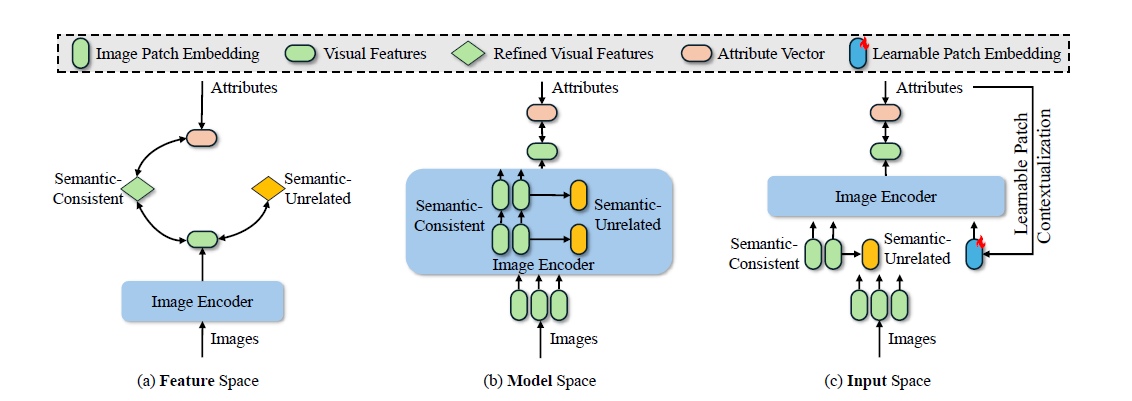
\includegraphics[width=\textwidth]{Image/Figure 1.PNG}
    \caption{Các phương pháp để giảm thiểu sự sai lệch ngữ nghĩa cho ZSL. (a) Các phương pháp tách rời loại bỏ thông tin không liên quan đến ngữ nghĩa trong không gian đặc trưng. (b) Các phương pháp hướng dẫn ngữ nghĩa tiến bộ loại bỏ các bản vá không liên quan đến ngữ nghĩa trong không gian mô hình. (c) SVIP của chúng tôi xác định các bản vá hình ảnh không liên quan đến ngữ nghĩa ở vị trí đầu vào và thay thế chúng bằng các bản vá thị giác được bối cảnh hóa về mặt ngữ nghĩa.}
    \label{fig:approaches}
\end{figure*}

năng học biểu diễn mạnh mẽ của Vision Transformers (ViTs) \cite{19, 66}, các nhà nghiên cứu trong cộng đồng ZSL đang chuyển sang thiết kế các phương pháp dựa trên ViT \cite{4, 17, 32}. Hành vi mô hình hóa bản vá cho phép xác định các bản vá không liên quan đến ngữ nghĩa. Như trong Hình \ref{fig:approaches}(b), ZSLViT \cite{4} loại bỏ dần các token thị giác không ánh xạ tới ngữ nghĩa trong không gian mô hình. Tuy nhiên, nghiên cứu đã chỉ ra rằng các đặc trưng ngữ nghĩa có thể bị loãng ở các lớp sâu hơn của ViT \cite{40}, khiến cho thông tin không liên quan đến ngữ nghĩa dễ dàng tồn tại và có khả năng làm ô nhiễm các đặc trưng thị giác cuối cùng.


Như trên, các phương pháp này hoặc loại bỏ các đặc trưng không liên quan đến ngữ nghĩa sau khi trích xuất các đặc trưng thị giác bị vướng víu, hoặc trong quá trình trích xuất các đặc trưng thị giác, chúng không hoàn toàn ngăn chặn các đặc trưng đó ảnh hưởng đến các biểu diễn đã học. Do đó, một câu hỏi nghiên cứu hấp dẫn được đặt ra: \textbf{Chúng ta có thể loại bỏ hoặc tái sử dụng một cách ưu tiên các bản vá không liên quan đến ngữ nghĩa ở giai đoạn đầu vào để tránh vướng víu chúng vào các đặc trưng đã học không?}

Để đạt được mục tiêu này, chúng tôi đề xuất \textbf{SVIP}, Semantically contextualized VIsual Patch, một framework dựa trên ViT được thiết kế để giảm thiểu thông tin không liên quan đến ngữ nghĩa và tăng cường sự lan truyền ngữ nghĩa-thị giác trong ZSL. Như được trình bày trong Hình \ref{fig:approaches}(c), không giống như các công trình trước đây cắt tỉa hoặc tinh chỉnh các đặc trưng sau khi chúng đã được trích xuất, SVIP xác định và bối cảnh hóa các bản vá này ngay từ đầu.

Cụ thể, để giải quyết vấn đề sai lệch ngữ nghĩa một cách toàn diện, chúng tôi đề xuất cơ chế lựa chọn bản vá tự giám sát nhằm học cách xác định các bản vá không liên quan đến ngữ nghĩa trong không gian đầu vào, tức là, trước khi đưa vào các khối transformer. Đặc biệt, chúng tôi tổng hợp các ma trận trọng số tự chú ý trên tất cả các khối transformer, mang lại sự hiểu biết ngữ nghĩa đáng tin cậy về tầm quan trọng của bản vá trong toàn bộ ViT. Để giảm thiểu tác động tiêu cực của các bản vá không liên quan đến ngữ nghĩa đối với các bản vá liên quan đến ngữ nghĩa, chúng tôi huấn luyện một bộ phân loại bản vá để xác định các bản vá đầu vào không liên quan đến ngữ nghĩa, sử dụng sự giám sát từ ma trận chú ý tổng hợp. Tại thời điểm kiểm tra, bộ phân loại bản vá có thể trực tiếp ngăn chặn các bản vá không liên quan đến ngữ nghĩa lan truyền vào quá trình trích xuất đặc trưng. Một khi các bản vá không liên quan đến ngữ nghĩa được xác định trong chuỗi đầu vào, một giải pháp đơn giản là loại bỏ chúng khỏi chuỗi đầu vào. Tuy nhiên, điều này có thể phá vỡ cấu trúc đối tượng trên hình ảnh. Thay vào đó, chúng tôi đề xuất che các bản vá không liên quan đến ngữ nghĩa bằng một bản vá ngữ cảnh có thể học được. Bản vá ngữ cảnh ngữ nghĩa được khởi tạo bằng các nhúng từ cấp thuộc tính cung cấp thông tin ngữ nghĩa phong phú. Các bản vá đầu vào được bối cảnh hóa này có thể tăng cường tương tác thị giác-ngữ nghĩa trong suốt quá trình trích xuất đặc trưng thị giác. Nhìn chung, những đóng góp của bài báo này là:
\begin{itemize}
    \item Chúng tôi giới thiệu Semantically contextualized VIsual Patch (SVIP), một framework dựa trên ViT để giải quyết vấn đề sai lệch ngữ nghĩa trong zero-shot learning. Nó nhấn mạnh việc xử lý sớm các bản vá không liên quan đến ngữ nghĩa để đạt được một không gian đặc trưng tập trung và rõ ràng hơn cho ZSL.
    \item Chúng tôi đề xuất một chiến lược lựa chọn bản vá tự giám sát để xác định các bản vá không liên quan đến ngữ nghĩa bằng cách sử dụng các điểm chú ý được tổng hợp từ ma trận trọng số tự chú ý trên các khối ViT. Chúng tôi đề xuất bối cảnh hóa ngữ nghĩa bản vá bằng cách đưa các nhúng từ cấp thuộc tính vào các bản vá không liên quan đến ngữ nghĩa, đảm bảo rằng thông tin ngữ nghĩa được tích hợp vào các biểu diễn thị giác từ các lớp ban đầu của transformer.
    \item SVIP đạt được kết quả hiệu suất hiện đại trên ba bộ dữ liệu ZSL tiêu chuẩn trên cả cài đặt ZSL và ZSL tổng quát, chứng tỏ hiệu quả trong việc giảm thiểu sự sai lệch ngữ nghĩa trong không gian đầu vào.
\end{itemize}
\section{Công trình liên quan}

Trong kỷ nguyên học sâu \cite{5, 15, 16, 31, 50, 52, 53, 54, 55, 56, 57, 62, 63, 65, 67, 68, 69, 70, 71}, mục tiêu cốt lõi trong ZSL \cite{7, 8, 9, 11, 14, 22, 23, 24, 25, 28, 42, 45, 58, 60} là tổng quát hóa kiến thức thị giác-ngữ nghĩa thu được từ các lớp đã thấy sang các lớp chưa thấy. Sự tổng quát hóa này dựa vào các bộ mô tả ngữ nghĩa, thường được biểu diễn dưới dạng thuộc tính \cite{21}, tài liệu \cite{20}, hoặc nhúng từ \cite{36}. Các phương pháp ZSL chính thống có thể được phân loại chung thành các phương pháp sinh (generative methods) và các phương pháp dựa trên nhúng (embedding-based methods). Các phương pháp ZSL sinh thường tổng hợp các đặc trưng thị giác chưa thấy từ các bộ mô tả ngữ nghĩa bằng cách sử dụng các mô hình sinh, cho phép các quy trình phân loại tiêu chuẩn kết hợp các mẫu huấn luyện tổng hợp. Các phương pháp này tận dụng các kiến trúc sinh khác nhau, bao gồm GANs \cite{45, 60, 73}, VAEs \cite{43, 51} và Normalizing Flows \cite{10, 12, 44}. Các phương pháp ZSL dựa trên nhúng nhằm mục đích học một ánh xạ trực tiếp từ không gian thị giác sang không gian ngữ nghĩa, liên kết các biểu diễn hình ảnh với các bộ mô tả lớp. Các phương pháp này thường tận dụng cơ chế chú ý để khoanh vùng các bộ mô tả ngữ nghĩa. Zhu và cộng sự \cite{74} đã giới thiệu một mạng lưới cục bộ hóa đa chú ý có hướng dẫn ngữ nghĩa để trích xuất các đặc trưng chi tiết cục bộ của các bản vá phân biệt. Xu và cộng sự \cite{61} đã đề xuất một mạng lưới nguyên mẫu thuộc tính, trong đó mỗi nguyên mẫu đại diện cho một khái niệm ngữ nghĩa cụ thể và được sử dụng làm bộ lọc 1x1 để tích chập các bản đồ đặc trưng từ ResNet101 nhằm tập trung vào vùng quan tâm. Công trình tiếp theo \cite{33} đã đề xuất sử dụng mô hình GloVe \cite{39} để trích xuất các véc-tơ ngữ nghĩa từ tên thuộc tính (ví dụ: "ngực trắng"), được sử dụng thêm để đại diện cho các nguyên mẫu thuộc tính. Gần đây hơn, Chen và cộng sự \cite{3} đã phát triển một mạng lưới chưng cất ngữ nghĩa tương hỗ để tinh chỉnh sự liên kết giữa các đặc trưng thị giác và ngữ nghĩa.

Mặc dù có những tiến bộ trong các phương pháp dựa trên sinh và nhúng, sự sai lệch ngữ nghĩa vẫn là một thách thức cơ bản trong ZSL \cite{1, 4, 6, 9, 27, 30}. Một số công trình cố gắng tách rời các đặc trưng liên quan đến ngữ nghĩa khỏi các đặc trưng không liên quan đến ngữ nghĩa. DLFZRL \cite{46} là công trình đầu tiên giới thiệu ZSL dựa trên sự tách rời, chia các biểu diễn hình ảnh thành các đặc trưng ngữ nghĩa, không ngữ nghĩa, và không phân biệt. RFF \cite{27} đã áp dụng tối thiểu hóa thông tin tương hỗ để loại bỏ các chi tiết thị giác dư thừa, trong khi SDGZSL \cite{9} sử dụng phân tích tương quan tổng thể để tách các thành phần nhất quán về mặt ngữ nghĩa và không liên quan đến ngữ nghĩa trong không gian đặc trưng. FREE \cite{1} đã tinh chỉnh các đặc trưng thị giác thông qua một mất mát trung tâm biên tự thích ứng để tăng cường sự liên kết ngữ nghĩa. Dis-VAE \cite{30} đã giới thiệu một chiến lược tái tổ hợp lô để chưng cất các đặc trưng cụ thể của danh mục để nhận dạng chính xác hơn. Phương pháp ZSLViT dựa trên ViT gần đây \cite{4} giới thiệu một framework ZSL dựa trên vision transformer giúp hợp nhất các token không liên quan đến ngữ nghĩa để cải thiện sự liên kết thị giác-ngữ nghĩa trong việc học các biểu diễn ZSL. Mặc dù có những nỗ lực trong việc giảm thiểu vấn đề sai lệch ngữ nghĩa trong không gian đặc trưng hoặc không gian mô hình, sức mạnh của những bản vá thị giác thử nghiệm không được chú ý trong cơ chế chú ý vẫn bị bỏ qua. Trong bài báo này, chúng tôi học cách xác định các bản vá thị giác không liên quan đến ngữ nghĩa ở không gian đầu vào và bối cảnh hóa chúng về mặt ngữ nghĩa, do đó cho phép chúng truyền bá thông tin ngữ nghĩa đến những bản vá quan trọng đó trong suốt các giai đoạn học đặc trưng thị giác.

\section{Phương pháp luận}

\subsection{Thiết lập vấn đề}
Cho $D^s = \{(x^s, y^s)\}_{i=1}^{n_s}$ là một bộ dữ liệu đã thấy với các lớp $C^s$, trong đó mỗi hình ảnh $x \in \mathcal{X}$ có một nhãn tương ứng $y \in \mathcal{Y}^s$. Chúng ta cũng có một bộ dữ liệu chưa thấy $D^u = \{(x^u, y^u)\}_{j=1}^{n_u}$ với các lớp $C^u$. Theo thiết kế, $C^s$ và $C^u$ là rời rạc, đảm bảo $C^s \cap C^u = \emptyset$. Chúng ta ký hiệu thông tin ngữ nghĩa, tức là các thuộc tính, bằng $A = \{a_y\}_{y \in C^s \cup C^u}$ cho tất cả các lớp, trong khi chỉ có các lớp đã thấy là có sẵn để huấn luyện. Mục tiêu của chúng ta là huấn luyện một mô hình trên $D^s$ sao cho nó có thể nhận dạng chính xác các lớp trong $C^u$ tại thời điểm kiểm tra, mà không bao giờ thấy các ví dụ được gán nhãn cho $C^u$ trong quá trình huấn luyện.

\subsection{Động lực}
ZSL phụ thuộc vào việc căn chỉnh các đặc trưng thị giác với thông tin ngữ nghĩa. Tuy nhiên, thông tin không liên quan đến ngữ nghĩa trong không gian thị giác làm phức tạp sự căn chỉnh này. Nó tạo ra sự mơ hồ trong cách các thuộc tính ánh xạ đến các vùng hình ảnh có liên quan. Như thể hiện trong Hình \ref{fig:approaches}, các phương pháp hiện có loại bỏ thông tin không liên quan đến ngữ nghĩa trong (1) \textbf{không gian đặc trưng} (feature space), bằng cách xử lý sau các đặc trưng được trích xuất, hoặc (2) \textbf{không gian mô hình} (model space), bằng cách cắt bỏ các bản vá không liên quan trong các lớp khác nhau. Trong khi các chiến lược này phần nào ngăn chặn thông tin không liên quan đến ngữ nghĩa, chúng không loại bỏ hoàn toàn chúng. Do đó, nhiễu như vậy vẫn tồn tại trong các biểu diễn cuối
\begin{figure*}[t]
    \centering
    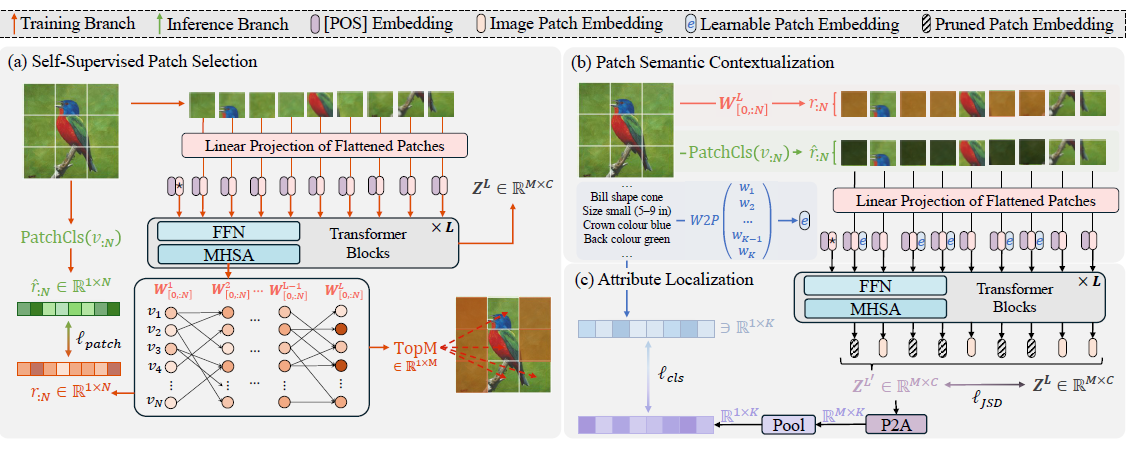
\includegraphics[width=\textwidth]{Image/Figure 2.PNG}
    \caption{Khung làm việc của SVIP được đề xuất của chúng tôi, bao gồm ba thành phần: (a) Lựa chọn bản vá Tự giám sát: chúng tôi tổng hợp các ma trận chú ý trong suốt các khối transformer để hướng dẫn việc huấn luyện bộ phân loại bản vá trong việc xác định các bản vá đầu vào không liên quan đến ngữ nghĩa. (b) Bối cảnh hóa Ngữ nghĩa Bản vá: chúng tôi áp dụng các nhúng bản vá có thể học được được khởi tạo bằng các nhúng từ thuộc tính để bối cảnh hóa các bản vá không liên quan đến ngữ nghĩa. (c) Cục bộ hóa Thuộc tính: chúng tôi cục bộ hóa các giá trị thuộc tính bằng các nhúng bản vá đầu ra cuối cùng, thay vì token lớp.}
    \label{fig:approaches}
\end{figure*}
cùng.

Ngược lại, như thể hiện trong Hình \ref{fig:framework}, chúng tôi đề xuất xác định và lọc các bản vá không liên quan đến ngữ nghĩa trong \textbf{không gian đầu vào} (input space), trước khi nó lan truyền vào mô hình. Sự can thiệp sớm này bảo tồn một biểu diễn sạch hơn, mạch lạc hơn về mặt ngữ nghĩa trong suốt quá trình trích xuất đặc trưng. Do đó, quy trình ZSL tiếp theo có thể tập trung vào các tương tác thị giác-ngữ nghĩa có ý nghĩa và cải thiện nhận dạng lớp chưa thấy.

\subsection{Lựa chọn bản vá Tự giám sát (Self-Supervised Patch Selection)}
Để khoanh vùng các bản vá không liên quan đến ngữ nghĩa, chúng tôi đề xuất một cơ chế Lựa chọn bản vá Tự giám sát (Self-Supervised Patch Selection - SSPS) huấn luyện một bộ phân loại nhị phân để dự đoán điểm ngữ nghĩa của các bản vá hình ảnh, sử dụng sự chú ý tổng hợp từ transformer làm giám sát.

\textbf{Revisiting ViT.} Chúng tôi phân chia một hình ảnh $x \in \mathbb{R}^{H \times W \times C}$ thành $N$ bản vá $\{p_1, \dots, p_N\}$. Mỗi bản vá sau đó được làm phẳng và chiếu tuyến tính thành một nhúng bản vá:
\begin{equation}
\{v_1, \dots, v_N\} = \text{PatchEmb}(\{p_1, \dots, p_N\}),
\end{equation}
chúng tôi thêm một token lớp có thể học $v_{cls}$ và thêm các nhúng vị trí $E_{pos}$ để tạo thành chuỗi bản vá ban đầu:
\begin{equation}
Z^0 = [v_{cls}, v_1, \dots, v_N] + E_{pos}.
\end{equation}
Chuỗi bản vá này đi qua $L$ khối transformer:
\begin{equation}
Z^l = \text{TransformerBlock}^l(Z^{l-1}), l=1, \dots, L.
\end{equation}
tạo ra các đầu ra cuối cùng $Z^L = [z_{cls}, z_1, \dots, z_N]$. Ở đây, token lớp $z_{cls}$ được lấy làm biểu diễn toàn cục.

\textbf{Giám sát bản vá thông qua Tổng hợp Ma trận Chú ý.} Để ước tính điểm ngữ nghĩa của mỗi bản vá, chúng tôi thu thập các điểm chú ý từ các khối tự chú ý đa đầu (MHSA). Cho $T^l \in \mathbb{R}^{(N+1) \times (N+1)}$ là ma trận chú ý trong khối transformer thứ $l$ được tổng hợp trên tất cả các đầu chú ý. Chúng tôi tổng hợp các điểm chú ý này qua các lớp:
\begin{equation}
W^l = W^{l-1} + W^{l-1} \times T^l, l=1, \dots, L,
\end{equation}
trong đó $W^1 = T^1$. Ma trận tổng hợp $W^L$ cung cấp một cái nhìn toàn cục về tầm quan trọng của bản vá. Chúng tôi tiếp tục lấy hàng tương ứng với token lớp (chỉ số 0) để cung cấp điểm của mỗi bản vá: $r_i = W^L_{[0, i]}$, có thể dùng làm nhãn giả của các điểm ngữ nghĩa.
Sau đó, chúng tôi giới thiệu một bộ phân loại bản vá phụ để dự đoán điểm ngữ nghĩa của mỗi nhúng bản vá:
\begin{equation}
\hat{r}_i = \text{PatchCls}(v_i), i=1, \dots, N.
\end{equation}
Việc căn chỉnh $\hat{r}_i$ với $r_i$ có nguồn gốc từ sự chú ý cho phép mô hình học sự phân biệt bản vá ngữ nghĩa chi tiết với một mất mát entropy chéo nhị phân:
\begin{equation}
\mathcal{L}_{patch} = -\frac{1}{N} \sum_{i=1}^{N} [r_i \log(\hat{r}_i) + (1-r_i)\log(1-\hat{r}_i)].
\end{equation}
Thiết kế này được thúc đẩy bởi tính chất động của các điểm chú ý qua các lớp transformer. Như thể hiện trong Hình \ref{fig:attention_visualization}, chúng tôi trực quan hóa điểm chú ý của 49 bản vá trên 12 lớp transformer. Tầm quan trọng của các bản vá này không nhất quán qua các lớp khác nhau. Do đó, việc dựa vào một số lớp nhất định để xác định các bản vá không liên quan đến ngữ nghĩa có thể dẫn đến phân loại sai. Trong SSPS, chúng tôi tạo ra các nhãn giả mạnh mẽ hơn bằng cách tổng hợp các điểm chú ý trên tất cả các lớp.

\begin{figure}[t]
    \centering
    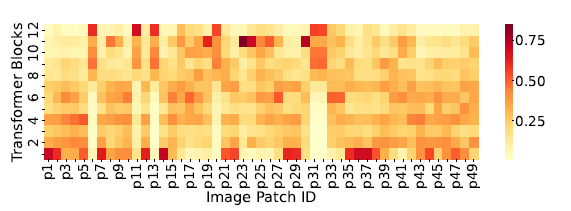
\includegraphics[width=0.9\columnwidth]{Image/Figure 3.PNG}
    \caption{Một trực quan hóa về trọng số chú ý của bản vá trên tất cả các lớp tự chú ý trong ViT.}
    \label{fig:attention_visualization_2}
\end{figure}

\subsection{Bối cảnh hóa Ngữ nghĩa Bản vá (Patch Semantic Contextualization)}
Mặc dù việc loại bỏ các bản vá không liên quan đến ngữ nghĩa có thể chỉ bảo tồn các bản vá thông tin, nó có thể phá vỡ cấu trúc đối tượng. Thay vào đó, chúng tôi đề xuất Bối cảnh hóa Ngữ nghĩa Bản vá (Patch Semantic Contextualization - PSC) để bối cảnh hóa các bản vá này với thông tin cấp thuộc tính, biến đổi các nhúng của chúng để căn chỉnh tốt hơn với ngữ nghĩa.

\textbf{Nhúng bản vá có thể học.} Chúng tôi định nghĩa một nhúng bản vá có thể học $e$ được khởi tạo từ các véc-tơ từ \cite{39}. Cho $\{w_1, \dots, w_K\}$ là các nhúng từ cho $K$ thuộc tính (ví dụ: màu sắc, hình dạng). Chúng được tổng hợp thông qua một lớp chiếu Word-to-Patch (W2P):
\begin{equation}
e = \text{W2P}(w_1, \dots, w_K).
\end{equation}
Tiếp theo, chúng tôi xác định các bản vá có điểm dự đoán $\hat{r}_i$ vượt quá một ngưỡng hoặc xếp hạng trong top $M$:
\begin{equation}
S_M = \text{TopM}_{i \in \{1, \dots, N\}} \{\hat{r}_i, M\}.
\end{equation}
Sau đó, chúng tôi đưa $e$ vào mỗi bản vá được chọn như tiêm các nhúng vị trí:
\begin{equation}
Z^{0'} = [v_{cls}, v'_1, \dots, v'_N] + E_{pos}, \quad v'_i = 
\begin{cases}
    v_i + e, & \text{nếu } i \in S_M \\
    v_i, & \text{khác}.
\end{cases}
\end{equation}
Bởi vì các nhúng bản vá được cập nhật $v'_i$ mang thông tin ngữ nghĩa cấp thuộc tính trong không gian đầu vào, điều này có thể tăng cường tương tác thị giác-ngữ nghĩa trong suốt các khối transformer.

\subsection{Cục bộ hóa Thuộc tính (Attribute Localization)}
Mặc dù token lớp cuối cùng $z_{cls}$ có thể nắm bắt biểu diễn toàn cục, các bản vá liên quan đến ngữ nghĩa có thể giúp cục bộ hóa các thuộc tính. Cho $Z^{L'} = \{z'_i | i \in S_M\}$ là các biểu diễn cuối cùng của top $M$ bản vá liên quan đến ngữ nghĩa. Chúng tôi học một hàm chiếu Patch-to-Attribute (P2A) để ánh xạ các nhúng bản vá $Z^{L'} \in \mathbb{R}^{M \times C}$ vào không gian thuộc tính: $\hat{A} = \text{P2A}(Z^{L'}) \in \mathbb{R}^{M \times K}$, trong đó $K$ là số lượng thuộc tính mô tả một danh mục. Một hoạt động gộp tối đa (max pooling) sau đó được áp dụng trên các nhúng thuộc tính bản vá này:
\begin{equation}
\hat{a} = \text{MaxPool}(\hat{A}),
\end{equation}
xác định bản vá phù hợp nhất cho mỗi thuộc tính. Do đó, mô hình học cách tập trung khi dự đoán một giá trị thuộc tính. Xác suất phân loại tuân theo một SoftMax tiêu chuẩn trên các điểm tương đồng cosine:
\begin{equation}
p(y|Z^0) = \frac{\exp(\sigma \cdot \cos(\hat{a}, a_y))}{\sum_{\tilde{y} \in \mathcal{Y}^s} \exp(\sigma \cdot \cos(\hat{a}, a_{\tilde{y}}))},
\end{equation}
trong đó $a_y$ là véc-tơ thuộc tính của một lớp đã thấy $y$ và $\sigma$ là nhiệt độ để điều chỉnh các điểm tương đồng cosine.

\subsection{Tối ưu hóa và Suy luận Mô hình}
\textbf{Tối ưu hóa.} Chúng tôi truyền mỗi mẫu qua các khối transformer hai lần: một lần với các bản vá gốc $Z^0$ và một lần với các bản vá được bối cảnh hóa $Z^{0'}$. Do đó, mất mát phân loại của chúng tôi tổng hợp cả hai dự đoán:
\begin{equation}
\mathcal{L}_{cls} = -\log p(y|Z^0) - \log p(y|Z^{0'}).
\end{equation}
Để ổn định việc huấn luyện cho các bản vá được bối cảnh hóa, chúng tôi áp dụng phân kỳ Jensen-Shannon (Jensen-Shannon divergence) giữa hai phân phối đầu ra:
\begin{equation}
\mathcal{L}_{JSD} = \frac{1}{2} D_{KL}(p(y|Z^0) \parallel \bar{p}) + \frac{1}{2} D_{KL}(p(y|Z^{0'}) \parallel \bar{p})
\end{equation}
với $\bar{p} = \frac{1}{2}(p(y|Z^0) + p(y|Z^{0'}))$.
Nhìn chung, mục tiêu huấn luyện được định nghĩa là:
\begin{equation}
\mathcal{L}_{overall} = \mathcal{L}_{cls} + \lambda_1 \mathcal{L}_{JSD} + \lambda_2 \mathcal{L}_{patch},
\end{equation}
trong đó $\lambda_1$ và $\lambda_2$ là các hệ số mất mát. Toàn bộ quá trình huấn luyện được minh họa trong Thuật toán 1.

\textbf{Suy luận Zero-Shot.} Đầu tiên, chúng tôi phân vùng một hình ảnh thử nghiệm thành nhiều bản vá và chiếu chúng thành các nhúng bản vá tương ứng bằng Eq. (1). Sau đó, chúng tôi xác định các bản vá không liên quan đến ngữ nghĩa bằng bộ phân loại bản vá đã học bằng Eq. (5). Trong khi tất cả các nhúng bản vá được áp dụng với các nhúng vị trí, chỉ những bản vá không liên quan đến ngữ nghĩa mới được áp dụng với các nhúng bản vá ngữ nghĩa đã học như trong Eq. (9). Các nhúng bản vá này được đưa vào các khối transformer để cục bộ hóa thuộc tính hơn nữa. Cuối cùng, chúng tôi suy ra nhãn lớp chưa thấy được dự đoán bằng Eq. (11).

\section{Thực nghiệm}

\subsection{Thiết lập thực nghiệm}
\textbf{Bộ dữ liệu.} Chúng tôi tiến hành các thí nghiệm trên ba bộ dữ liệu benchmark cho zero-shot learning, đó là CUB \cite{49}, AwA2 \cite{29}, SUN \cite{38}. Cụ thể, CUB chứa 11,788 hình ảnh trên 200 loài chim, mỗi loài được chú thích với 312 thuộc tính. AwA2 bao gồm 37,322 hình ảnh trên 50 loài động vật được mô tả bởi 85 thuộc tính. SUN bao gồm 14,340 hình ảnh từ 717 lớp cảnh được chụp với 102 thuộc tính. Chúng tôi sử dụng các phân chia huấn luyện được đề xuất trong \cite{60}, các lớp đã thấy/chưa thấy được chia thành 150/50, 40/10 và 645/72 tương ứng.

\textbf{Đánh giá.} Theo \cite{59}, chúng tôi đo lường độ chính xác top-1 trong cả hai cài đặt zero-shot learning (ZSL) và generalized zero-shot learning (GZSL). Trong cài đặt ZSL, chúng tôi chỉ đánh giá độ chính xác của các mẫu thử nghiệm trong các lớp chưa thấy. Trong cài đặt GZSL, chúng tôi tính toán độ chính xác của các mẫu thử nghiệm từ cả hai lớp đã thấy (ký hiệu là S) và chưa thấy (ký hiệu là U). Để đánh giá hiệu suất chung, trung bình điều hòa (harmonic mean) giữa các lớp đã thấy và chưa thấy là một số liệu đánh giá chính trong cài đặt GZSL, được định nghĩa là $H = (2 \times S \times U) / (S + U)$.

\textbf{Triển khai.} Mô hình của chúng tôi được triển khai dựa trên mô hình ViT-base \cite{47} (kích thước đầu vào hình ảnh: 224$\times$224), được huấn luyện trước trên ImageNet-1k làm cơ sở và để khởi tạo, điều này nhất quán với các phương pháp ZSL dựa trên ViT hiện có. ViT-base có số lượng bản vá mặc định là 196, nhưng để hiệu quả tính toán, chúng tôi tổng hợp mỗi 4 (2$\times$2) bản vá thành một, cho ra 49 bản vá.

\subsection{Kết quả chính}
\textbf{Hiệu quả đối với sự sai lệch ngữ nghĩa.} Để cho thấy hiệu quả của SVIP trong việc giải quyết sự sai lệch ngữ nghĩa, chúng tôi so sánh SVIP với các phương pháp nhằm đạt được điều này trong không gian đặc trưng (RFF \cite{27}, SDGZSL \cite{9}, Dis-VAE \cite{30}) hoặc ở cấp độ mô hình (ZSLViT \cite{4}). Như được trình bày trong Bảng 1, phương pháp của chúng tôi đạt được hiệu suất vượt trội trong cả hai cài đặt ZSL và GZSL trên ba bộ dữ liệu benchmark, ngoại trừ hiệu suất ZSL trên AwA2 mà chúng tôi đạt được hiệu suất tương đương. Những cải tiến này xác nhận rằng việc lọc các bản vá không liên quan ở giai đoạn đầu vào là rất hiệu quả để tăng cường sự liên kết thị giác-ngữ nghĩa và nâng cao độ chính xác nhận dạng zero-shot tổng thể.

\textbf{So sánh với các Backbone CNN.} Tiếp theo, chúng tôi so sánh SVIP với một nhóm các phương pháp sử dụng ResNet101 làm backbone của chúng (khối trên của Bảng 1). Cụ thể, các phương pháp như APN \cite{61}, GEM \cite{33}, MSDN \cite{3}, Dis-VAE, và ICCE đều hoạt động trên các đặc trưng toàn cục được trích xuất từ CNN để căn chỉnh không gian thị giác và ngữ nghĩa cho zero-shot learning. Mặc dù chúng có hiệu quả trên một số bộ dữ liệu nhất định, SVIP của chúng tôi đạt được kết quả hiệu suất hiện đại một cách nhất quán trên CUB, AwA2 và SUN. Đáng chú ý, SVIP đạt được giá trị H là 75.0\% trên CUB, 74.9\% trên AwA2 và 50.7\% trên SUN, vượt qua tất cả các phương pháp dựa trên ResNet101 cạnh tranh. Những kết quả này chứng tỏ hiệu quả của SVIP trong việc nắm bắt các tín hiệu ngữ nghĩa chi tiết trong khi vẫn duy trì khả năng phân biệt mạnh mẽ cho cả các lớp đã thấy (S) và chưa thấy (U).

\textbf{So sánh với các Backbone ViT.} Tiếp theo, chúng tôi so sánh SVIP với các phương pháp gần đây với ViT làm backbone, bao gồm các phương pháp dựa trên ngôn ngữ (CLIP \cite{41}, CoOp \cite{72}, I2DFormer \cite{34}, I2MV \cite{35}), các phương pháp dựa trên thuộc tính (DUET \cite{13}, ZSLViT \cite{4}). Nói chung, các phương pháp dựa trên ViT được hưởng lợi từ các cơ chế chú ý trên các nhúng bản vá, nhưng chúng thường thiếu sự giám sát rõ ràng cho các bản vá không liên quan đến ngữ nghĩa. Như đã trình bày, SVIP mang lại hiệu suất tốt nhất về độ chính xác chưa thấy (U) trên CUB (72.1\%) và SUN (53.7\%), cũng như trung bình điều hòa hàng đầu trên cả hai bộ dữ liệu. Trên AwA2, phương pháp của chúng tôi cũng cho thấy kết quả cạnh tranh, chứng tỏ khả năng thích ứng của lý luận thuộc tính cục bộ của SVIP trên một loạt các miền thị giác.

\textbf{Nghiên cứu cắt bỏ (Ablation Study).} Chúng tôi tiến hành một nghiên cứu cắt bỏ để phân tích sự đóng góp của từng thành phần trong SVIP (Bảng 2). Baseline (ViT) sử dụng một lớp tuyến tính đơn giản trên token lớp mà không có các hoạt động cấp bản vá, mang lại hiệu suất thấp nhất. SVIP không có SSPS loại bỏ Lựa chọn bản vá Tự giám sát, áp dụng các bản vá ngữ nghĩa một cách bừa bãi, dẫn đến sụt giảm đáng kể, làm nổi bật sự cần thiết của việc lựa chọn bản vá có mục tiêu. SVIP không có PSC loại bỏ trực tiếp các bản vá không liên quan đến ngữ nghĩa thay vì bối cảnh hóa chúng, điều này làm gián đoạn một chút cấu trúc đối tượng và làm giảm hiệu suất. SVIP không có JSD loại trừ phân kỳ Jensen-Shannon, làm giảm sự ổn định huấn luyện và độ chính xác tổng thể. SVIP không có W2P thay thế các nhúng từ bằng các nhúng bản vá được khởi tạo ngẫu nhiên, dẫn đến sự suy giảm liên kết ngữ nghĩa. SVIP không có P2A loại bỏ ánh xạ Patch-to-Attribute, buộc phải dựa vào token lớp, điều này làm suy yếu độ chính xác của lớp chưa thấy.

\textbf{Độ nhạy của siêu tham số.} Trong một loạt các thí nghiệm, chúng tôi khảo sát ảnh hưởng của bốn siêu tham số đến hiệu suất của phương pháp được đề xuất của chúng tôi. Hình \ref{fig:hyperparameter} (a) cho thấy ảnh hưởng của việc thay đổi số lượng bản vá được bảo tồn M từ 49 đến 35. Hiệu suất bão hòa xảy ra ở khoảng 40, và số lượng bản vá lớn hơn có xu hướng làm giảm hiệu suất do cắt tỉa quá mức các bản vá liên quan đến ngữ nghĩa. Hình \ref{fig:hyperparameter} (b) chứng minh rằng Phân kỳ JS là một siêu tham số khá nhạy cảm, đạt hiệu suất tốt nhất ở mức 1. Trong Hình \ref{fig:hyperparameter} (c), chúng tôi thay đổi hệ số mất mát cho bộ phân loại bản vá $\lambda_2$ và thấy rằng cả ZSL và GZSL đều đạt hiệu suất tốt nhất ở mức 3. Trong Hình \ref{fig:hyperparameter} (d), chúng tôi thấy rằng thang nhiệt độ có tác động đáng kể đến sự thay đổi hiệu suất, đạt đỉnh ở mức 5.

\begin{table*}[t]
    \centering
    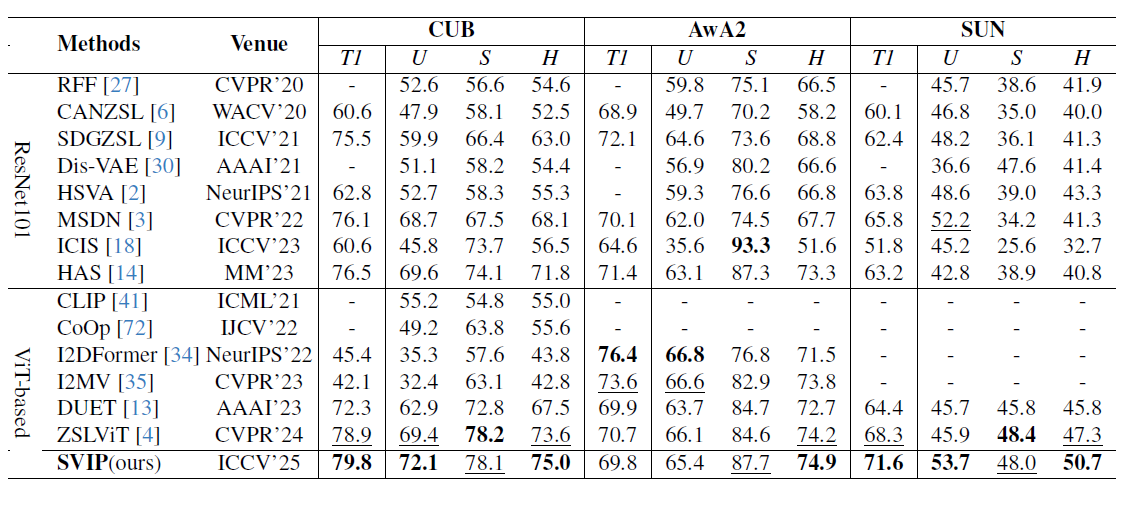
\includegraphics[width=\textwidth]{Image/Table 1.PNG}
    \caption{So sánh các mô hình ZSL và GZSL hiện đại trên ba bộ dữ liệu benchmark. Đối với ZSL, kết quả được báo cáo là độ chính xác top-1 trung bình (T1). Đối với GZSL, chúng tôi báo cáo độ chính xác top-1 cho các lớp chưa thấy (U) và đã thấy (S), cùng với trung bình điều hòa của chúng (H). Các kết quả tốt nhất và tốt thứ hai được tô đậm và gạch chân, tương ứng.}
    \label{tab:main_results}
\end{table*}

\begin{table*}[t]
    \centering
    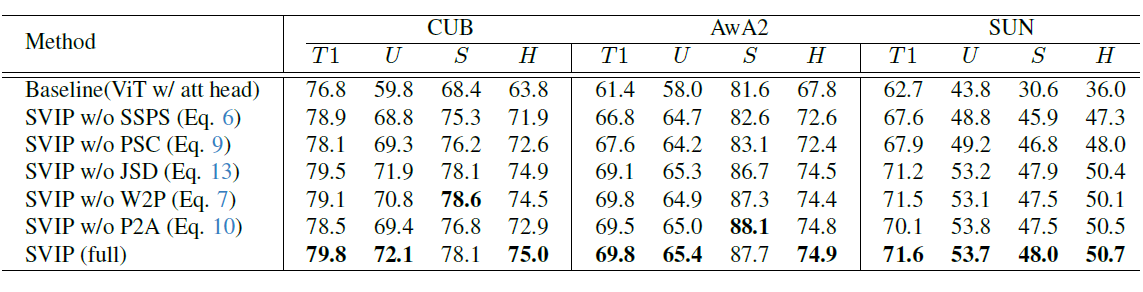
\includegraphics[width=\textwidth]{Image/Table 2.PNG}
    \caption{Phân tích các thành phần khác nhau trong SVIP.}
    \label{tab:ablation}
\end{table*}

\begin{figure*}[t]
    \centering
    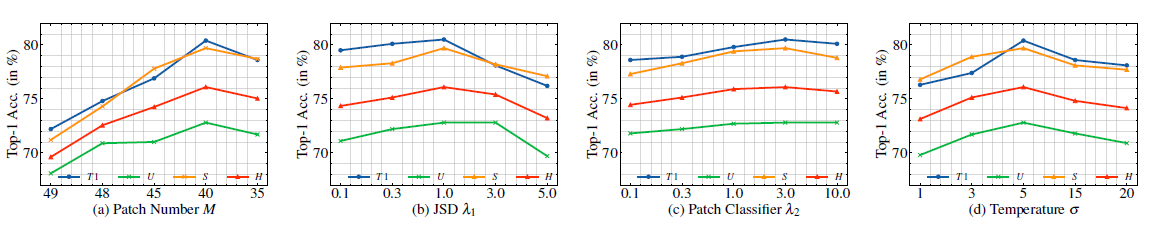
\includegraphics[width=\textwidth]{Image/Figure 4.PNG}
    \caption{Độ nhạy của siêu tham số trên bộ dữ liệu CUB. Trục ngang chỉ ra các siêu tham số thay đổi cho (a) số lượng bản vá được bảo tồn M, (b) hệ số mất mát JSD $\lambda_1$, (c) hệ số mất mát bộ phân loại bản vá $\lambda_2$, và (d) nhiệt độ logits $\sigma$.}
    \label{fig:hyperparameter}
\end{figure*}

\subsection{Nghiên cứu Định tính}
\textbf{Cục bộ hóa Thuộc tính (Attribute Localization).} Chúng tôi trình bày các bản đồ chú ý (tức là, lớp trước hoạt động gộp tối đa) trong Hình \ref{fig:attention_maps}, cho các thuộc tính được chọn ngẫu nhiên trên ba hình ảnh ví dụ từ bộ dữ liệu CUB. Các bản đồ chú ý được tạo ra bằng cách áp dụng các hoạt động gộp tối đa cho đầu ra của mô hình, làm nổi bật các vùng mà mô hình đang tập trung vào cho mỗi thuộc tính. Các vùng được che bằng sọc chéo được xác định là các bản vá không liên quan đến ngữ nghĩa và do đó không được xem xét để cục bộ hóa thuộc tính. Phương pháp cơ sở ViT tập trung vào nhiều bản vá không chính xác được phân loại là các bản vá không liên quan đến ngữ nghĩa trong SVIP, điều này chứng tỏ sự hữu ích của SSPS.

\textbf{Trực quan hóa Dự đoán Thuộc tính.} Hình \ref{fig:tsne_visualization} trình bày một trực quan hóa t-SNE của các véc-tơ thuộc tính được dự đoán từ ViT cơ sở (trái) và SVIP được đề xuất của chúng tôi (phải) trên các hình ảnh của 20 lớp được chọn ngẫu nhiên từ tập hợp chưa thấy của bộ dữ liệu CUB. Trong ViT cơ sở Hình \ref{fig:tsne_visualization}(a), các cụm xuất hiện kém khác biệt hơn, với các điểm thuộc tính chồng chéo và phân tán, như được chỉ ra bởi các vòng tròn đứt nét màu đỏ. Điều này cho thấy rằng thông tin không liên quan đến ngữ nghĩa làm gián đoạn các biểu diễn đã học, dẫn đến sự liên kết thị giác-ngữ nghĩa yếu hơn. Ngược lại, SVIP trong Hình \ref{fig:tsne_visualization}(b) cho thấy các cụm nhỏ gọn và được phân tách rõ ràng hơn, trong đó các thuộc tính được phân định rõ ràng hơn. Các vòng tròn đứt nét màu đỏ làm nổi bật cách SVIP giảm sự mơ hồ về ngữ nghĩa, đảm bảo rằng các thuộc tính tương tự tạo thành các nhóm mạch lạc và có cấu trúc tốt hơn. Những kết quả này xác thực hiệu quả của việc lựa chọn bản vá tự giám sát và bối cảnh hóa ngữ nghĩa trong việc cải thiện.

\textbf{Trực quan hóa Đặc trưng của Bộ phân loại Bản vá.} Hình \ref{fig:patch_visualization} minh họa cách phương pháp của chúng tôi lựa chọn và bối cảnh hóa các bản vá không liên quan đến ngữ nghĩa. Trong (a), mỗi hình ảnh chim được phân vùng thành các bản vá, và những bản vá được coi là không liên quan sẽ được tô bóng (sọc chéo). Việc lọc ở giai đoạn đầu này đảm bảo rằng mô hình tập trung vào các thuộc tính quan trọng để nhận dạng chim (ví dụ: các mẫu màu hoặc hình dạng đặc biệt). Trong (b), chúng tôi sử dụng t-SNE để trực quan hóa các nhúng trong lớp trung gian của bộ phân loại bản vá trong không gian hai chiều. Chúng tôi quan sát thấy rằng các bản vá không liên quan đến ngữ nghĩa cụm lại với nhau như được chỉ ra trong các hộp giới hạn màu đỏ, trong khi các bản vá ghi lại các đặc điểm có liên quan về mặt ngữ nghĩa thì phân tán hơn. Sự tách biệt này chứng thực khả năng của bộ phân loại bản vá của chúng tôi trong việc bảo tồn các tín hiệu thị giác có ý nghĩa và triệt tiêu thông tin không liên quan.

\begin{figure*}[t]
    \centering
    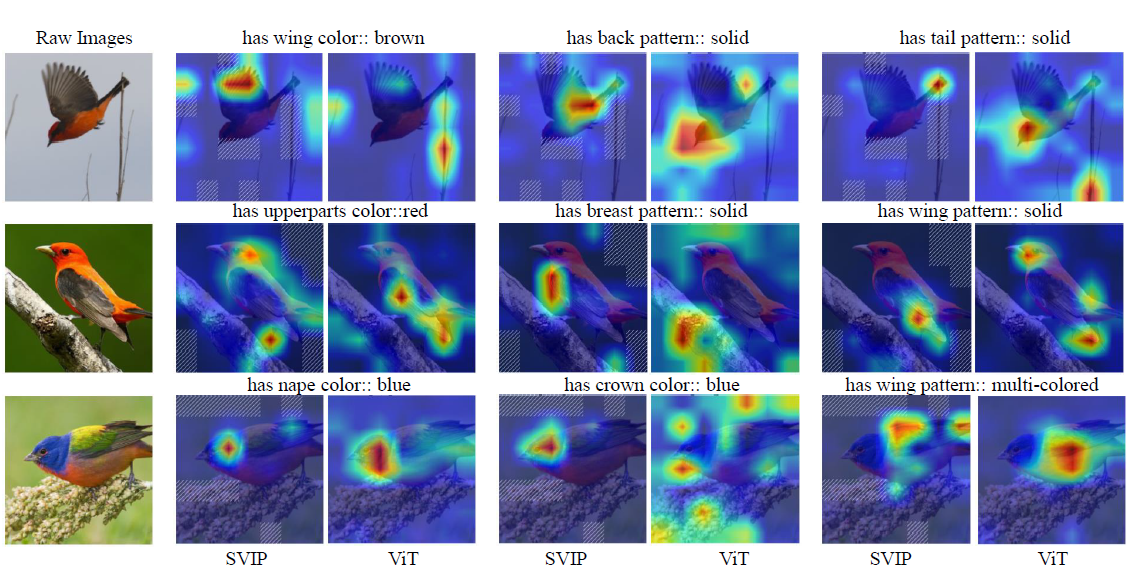
\includegraphics[width=\textwidth]{Image/Figure 5.PNG}
    \caption{Trực quan hóa các bản đồ chú ý thuộc tính được dự đoán trên ba mẫu thử nghiệm ngẫu nhiên của bộ dữ liệu CUB.}
    \label{fig:attention_maps}
\end{figure*}

\begin{figure*}[t]
    \centering
    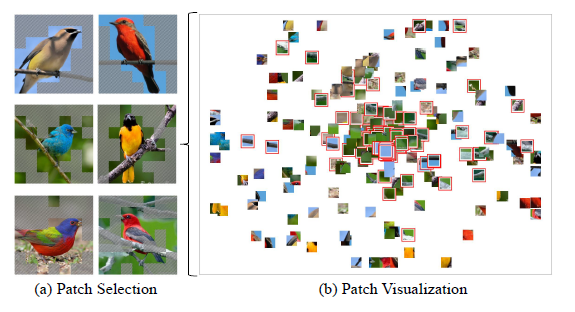
\includegraphics[width=\textwidth]{Image/Figure 6.PNG}
    \caption{(a) Hình ảnh ví dụ với các bản vá không liên quan đến ngữ nghĩa được che. (b) Trực quan hóa t-SNE của các bản vá hình ảnh, trong đó các hộp giới hạn màu đỏ chỉ ra các bản vá không liên quan về mặt ngữ nghĩa.}
    \label{fig:patch_visualization}
\end{figure*}

\begin{figure*}[t]
    \centering
    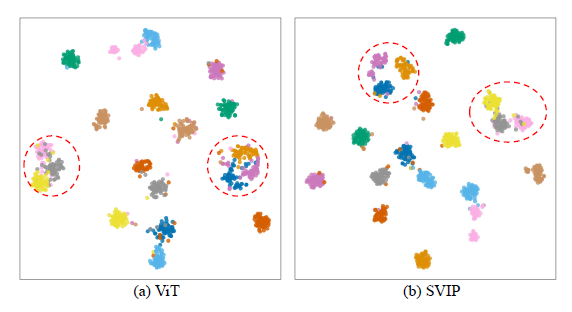
\includegraphics[width=0.9\textwidth]{Image/Figure 7.PNG}
    \caption{Trực quan hóa t-SNE của các véc-tơ thuộc tính được dự đoán từ (a) ViT cơ sở và (b) SVIP được đề xuất của chúng tôi.}
    \label{fig:tsne_visualization}
\end{figure*}

\section{Kết luận}

Trong bài báo này, chúng tôi đã giới thiệu một framework mới dựa trên ViT cho ZSL nhằm tăng cường sự liên kết thị giác-ngữ nghĩa bằng cách giải quyết vấn đề sai lệch ngữ nghĩa ở không gian đầu vào. Phương pháp của chúng tôi bao gồm hai thành phần chính: lựa chọn bản vá tự giám sát, tận dụng các điểm chú ý tổng hợp để xác định và loại bỏ các bản vá không liên quan đến ngữ nghĩa, và Bối cảnh hóa Ngữ nghĩa, thay thế các bản vá này bằng các nhúng có thể học được và nhận biết thuộc tính. Các thử nghiệm sâu rộng trên các bộ dữ liệu ZSL tiêu chuẩn đã chứng minh rằng phương pháp của chúng tôi đạt được kết quả hiệu suất hiện đại. Công trình của chúng tôi nhấn mạnh tầm quan trọng của việc tinh chỉnh ngữ nghĩa ở giai đoạn đầu trong ZSL và đề xuất các hướng đi mới để tích hợp các tiên nghiệm ngữ nghĩa vào các mô hình thị giác dựa trên transformer. Công việc trong tương lai sẽ khám phá các chiến lược thích ứng để lựa chọn và bối cảnh hóa bản vá, cho phép mô hình điều chỉnh linh hoạt dựa trên các đặc điểm của bộ dữ liệu.

\section*{Lời cảm ơn}
Công trình này được hỗ trợ bởi Hội đồng Nghiên cứu Úc (Australian Research Council) trong khuôn khổ của Dự án Khám phá (Discovery Project) (Số DP240101814).

\begin{thebibliography}{99}
\bibitem{1} Shiming Chen, Wenjie Wang, Beihao Xia, Qinmu Peng, Xinge You, Feng Zheng, and Ling Shao. Free: Feature refinement for generalized zero-shot learning. In ICCV, 2021.
\bibitem{2} Shiming Chen, Guosen Xie, Yang Liu, Qinmu Peng, Baigui Sun, Hao Li, Xinge You, and Ling Shao. Hsva: Hierarchical semantic-visual adaptation for zero-shot learning. In NeurIPS, 2021.
\bibitem{3} Shiming Chen, Ziming Hong, Guo-Sen Xie, Wenhan Yang, Qinmu Peng, Kai Wang, Jian Zhao, and Xinge You. Msdn: Mutually semantic distillation network for zero-shot learning. In CVPR, 2022.
\bibitem{4} Shiming Chen, Wenjin Hou, Salman Khan, and Fahad Shahbaz Khan. Progressive semantic-guided vision transformer for zero-shot learning. In CVPR, 2024.
\bibitem{5} Yudong Chen, Sen Wang, Jianglin Lu, Zhi Chen, Zheng Zhang, and Zi Huang. Local graph convolutional networks for cross-modal hashing. In ACM MM, 2021.
\bibitem{6} Zhi Chen, Jingjing Li, Yadan Luo, Zi Huang, and Yang Yang. Canzsl: Cycle-consistent adversarial networks for zero-shot learning from natural language. In WACV, 2020.
\bibitem{7} Zhi Chen, Sen Wang, Jingjing Li, and Zi Huang. Rethinking generative zero-shot learning: An ensemble learning perspective for recognising visual patches. In ACM MM, 2020.
\bibitem{8} Zhi Chen, Zi Huang, Jingjing Li, and Zheng Zhang. Entropy-based uncertainty calibration for generalized zero-shot learning. In ADC, 2021.
\bibitem{9} Zhi Chen, Yadan Luo, Ruihong Qiu, Sen Wang, Zi Huang, Jingjing Li, and Zheng Zhang. Semantics disentangling for generalized zero-shot learning. In ICCV, 2021.
\bibitem{10} Zhi Chen, Yadan Luo, Sen Wang, Ruihong Qiu, Jingjing Li, and Zi Huang. Mitigating generation shifts for generalized zero-shot learning. In ACM MM, 2021.
\bibitem{11} Zhi Chen, Yadan Luo, Sen Wang, Jingjing Li, and Zi Huang. Federated zero-shot learning for visual recognition. arXiv preprint arXiv:2209.01994, 2022.
\bibitem{12} Zhi Chen, Yadan Luo, Sen Wang, Jingjing Li, and Zi Huang. Gsmflow: Generation shifts mitigating flow for generalized zero-shot learning. IEEE Transactions on Multimedia, 2022.
\bibitem{13} Zhuo Chen, Yufeng Huang, Jiaoyan Chen, Yuxia Geng, Wen Zhang, Yin Fang, Jeff Z Pan, and Huajun Chen. Duet: Cross-modal semantic grounding for contrastive zero-shot learning. In AAAI, 2023.
\bibitem{14} Zhi Chen, Pengfei Zhang, Jingjing Li, Sen Wang, and Zi Huang. Zero-shot learning by harnessing adversarial samples. In ACM MM, 2023.
\bibitem{15} Zhi Chen, Tianqi Wei, Zecheng Zhao, Jia Syuen Lim, Yadan Luo, Hu Zhang, Xin Yu, Scott Chapman, and Zi Huang. Cf-prnet: Coarse-to-fine prototype refining network for point cloud completion and reconstruction. arXiv preprint arXiv:2409.08443, 2024.
\bibitem{16} Zhi Chen, Zecheng Zhao, Yadan Luo, and Zi Huang. Fastedit: Fast text-guided single-image editing via semantic-aware diffusion fine-tuning. arXiv preprint arXiv:2408.03355, 2024.
\bibitem{17} De Cheng, Gerong Wang, Bo Wang, Qiang Zhang, Jungong Han, and Dingwen Zhang. Hybrid routing transformer for zero-shot learning. Pattern Recognition, 2023.
\bibitem{18} Anders Christensen, Massimiliano Mancini, A Koepke, Ole Winther, and Zeynep Akata. Image-free classifier injection for zero-shot classification. In ICCV, 2023.
\bibitem{19} Alexey Dosovitskiy. An image is worth 16x16 words: Transformers for image recognition at scale. arXiv preprint arXiv:2010.11929, 2020.
\bibitem{20} Mohamed Elhoseiny, Babak Saleh, and Ahmed Elgammal. Write a classifier: Zero-shot learning using purely textual descriptions. In ICCV, 2013.
\bibitem{21} Ali Farhadi, Ian Endres, Derek Hoiem, and David Forsyth. Describing objects by their attributes. In CVPR, 2009.
\bibitem{22} Jingcai Guo and Song Guo. A novel perspective to zero-shot learning: Towards an alignment of manifold structures via semantic feature expansion. IEEE Transactions on Multimedia, 2020.
\bibitem{23} Jingcai Guo, Song Guo, Qihua Zhou, Ziming Liu, Xiaocheng Lu, and Fushuo Huo. Graph knows unknowns: Reformulate zero-shot learning as sample-level graph recognition. In AAAI, 2023.
\bibitem{24} Jingcai Guo, Zhijie Rao, Zhi Chen, Song Guo, Jingren Zhou, and Dacheng Tao. On the element-wise representation and reasoning in zero-shot image recognition: A systematic survey. arXiv preprint arXiv:2408.04879, 2024.
\bibitem{25} Jingcai Guo, Zhijie Rao, Zhi Chen, Jingren Zhou, and Dacheng Tao. Fine-grained zero-shot learning: Advances, challenges, and prospects. arXiv preprint arXiv:2401.17766, 2024.
\bibitem{26} Kai Han, Yunhe Wang, Hanting Chen, Xinghao Chen, Jianyuan Guo, Zhenhua Liu, Yehui Tang, An Xiao, Chunjing Xu, Yixing Xu, et al. A survey on vision transformer. IEEE TPAMI, 2022.
\bibitem{27} Zongyan Han, Zhenyong Fu, and Jian Yang. Learning the redundancy-free features for generalized zero-shot object recognition. In CVPR, 2020.
\bibitem{28} E. Kodirov, T. Xiang, and S. Gong. Semantic autoencoder for zero-shot learning. In CVPR, 2017.
\bibitem{29} C. H. Lampert, H. Nickisch, and S. Harmeling. Attribute-based classification for zero-shot visual object categorization. IEEE TPAMI, 2013.
\bibitem{30} Xiangyu Li, Zhe Xu, Kun Wei, and Cheng Deng. Generalized zero-shot learning via disentangled representation. In AAAI, 2021.
\bibitem{31} Jia Syuen Lim, Zhuoxiao Chen, Zhi Chen, Mahsa Baktashmotlagh, Xin Yu, Zi Huang, and Yadan Luo. Dipex: Dispersing prompt expansion for class-agnostic object detection. In NeurIPS, 2024.
\bibitem{32} Man Liu, Feng Li, Chunjie Zhang, Yunchao Wei, Huihui Bai, and Yao Zhao. Progressive semantic-visual mutual adaption for generalized zero-shot learning. In CVPR, 2023.
\bibitem{33} Yang Liu, Lei Zhou, Xiao Bai, Yifei Huang, Lin Gu, Jun Zhou, and Tatsuya Harada. Goal-oriented gaze estimation for zero-shot learning. In CVPR, 2021.
\bibitem{34} Muhammad Ferjad Naeem, Yongqin Xian, Luc V Gool, and Federico Tombari. I2dformer: Learning image to document attention for zero-shot image classification. In NeurIPS, 2022.
\bibitem{35} Muhammad Ferjad Naeem, Muhammad Gul Zain Ali Khan, Yongqin Xian, Muhammad Zeshan Afzal, Didier Stricker, Luc Van Gool, and Federico Tombari. I2mvformer: Large language model generated multi-view document supervision for zero-shot image classification. In CVPR, 2023.
\bibitem{36} Mohammad Norouzi, Tomas Mikolov, Samy Bengio, Yoram Singer, Jonathon Shlens, Andrea Frome, Greg S Corrado, and Jeffrey Dean. Zero-shot learning by convex combination of semantic embeddings. arXiv preprint arXiv:1312.5650, 2013.
\bibitem{37} Mark Palatucci, Dean Pomerleau, Geoffrey E Hinton, and Tom M Mitchell. Zero-shot learning with semantic output codes. In NeurIPS, 2009.
\bibitem{38} Genevieve Patterson, Chen Xu, Hang Su, and James Hays. The sun attribute database: Beyond categories for deeper scene understanding. IJCV, 2014.
\bibitem{39} Jeffrey Pennington, Richard Socher, and Christopher D Manning. Glove: Global vectors for word representation. In EMNLP, 2014.
\bibitem{40} Zhen Qin, Xiaodong Han, Weixuan Sun, Dongxu Li, Lingpeng Kong, Nick Barnes, and Yiran Zhong. The devil in linear transformer. arXiv preprint arXiv:2210.10340, 2022.
\bibitem{41} Alec Radford, Jong Wook Kim, Chris Hallacy, Aditya Ramesh, Gabriel Goh, Sandhini Agarwal, Girish Sastry, Amanda Askell, Pamela Mishkin, Jack Clark, et al. Learning transferable visual models from natural language supervision. In ICML, 2021.
\bibitem{42} Bernardino Romera-Paredes and Philip Torr. An embarrassingly simple approach to zero-shot learning. In ICML, 2015.
\bibitem{43} Edgar Schonfeld, Sayna Ebrahimi, Samarth Sinha, Trevor Darrell, and Zeynep Akata. Generalized zero-and few-shot learning via aligned variational autoencoders. In CVPR, 2019.
\bibitem{44} Yuming Shen, Jie Qin, Lei Huang, Li Liu, Fan Zhu, and Ling Shao. Invertible zero-shot recognition flows. In ECCV, 2020.
\bibitem{45} Hongzu Su, Jingjing Li, Zhi Chen, Lei Zhu, and Ke Lu. Distinguishing unseen from seen for generalized zero-shot learning. In CVPR, 2022.
\bibitem{46} Bin Tong, Chao Wang, Martin Klinkigt, Yoshiyuki Kobayashi, and Yuuichi Nonaka. Hierarchical disentanglement of discriminative latent features for zero-shot learning. In CVPR, 2019.
\bibitem{47} Hugo Touvron, Matthieu Cord, Matthijs Douze, Francisco Massa, Alexandre Sablayrolles, and Hervé Jégou. Training data-efficient image transformers \& distillation through attention. In ICML, 2021.
\bibitem{48} Ashish Vaswani, Noam Shazeer, Niki Parmar, Jakob Uszkoreit, Llion Jones, Aidan N Gomez, Łukasz Kaiser, and Illia Polosukhin. Attention is all you need. In NeurIPS, 2017.
\bibitem{49} Catherine Wah, Steve Branson, Peter Welinder, Pietro Perona, and Serge Belongie. The caltech-ucsd birds-200-2011 dataset. 2011.
\bibitem{50} Tianqi Wang, Jingcai Guo, Depeng Li, and Zhi Chen. On the discrimination and consistency for exemplar-free class incremental learning. arXiv preprint arXiv:2501.15454, 2025.
\bibitem{51} Wenlin Wang, Yunchen Pu, Vinay Verma, Kai Fan, Yizhe Zhang, Changyou Chen, Piyush Rai, and Lawrence Carin. Zero-shot learning via class-conditioned deep generative models. In AAAI, 2018.
\bibitem{52} Zixin Wang, Yadan Luo, Peng-Fei Zhang, Sen Wang, and Zi Huang. Discovering domain disentanglement for generalized multi-source domain adaptation. In ICME, 2022.
\bibitem{53} Zixin Wang, Yadan Luo, Zhi Chen, Sen Wang, and Zi Huang. Cal-sfda: Source-free domain-adaptive semantic segmentation with differentiable expected calibration error. In ACM MM, 2023.
\bibitem{54} Zixin Wang, Yadan Luo, Liang Zheng, Zhuoxiao Chen, Sen Wang, and Zi Huang. In search of lost online test-time adaptation: A survey. IJCV, 2024.
\bibitem{55} Zixin Wang, Dong Gong, Sen Wang, Zi Huang, and Yadan Luo. Is less more? exploring token condensation as training-free adaptation for clip. In ICCV, 2025.
\bibitem{56} Tianqi Wei, Zhi Chen, Zi Huang, and Xin Yu. Benchmarking in-the-wild multimodal disease recognition and a versatile baseline. In ACM MM, 2024.
\bibitem{57} Tianqi Wei, Zhi Chen, Xin Yu, Scott Chapman, Paul Melloy, and Zi Huang. Plantseg: A large-scale in-the-wild dataset for plant disease segmentation. arXiv preprint arXiv:2409.04038, 2024.
\bibitem{58} Yongqin Xian, Bernt Schiele, and Zeynep Akata. Zero-shot learning-the good, the bad and the ugly. In CVPR, 2017.
\bibitem{59} Yongqin Xian, Christoph H Lampert, Bernt Schiele, and Zeynep Akata. Zero-shot learning-a comprehensive evaluation of the good, the bad and the ugly. IEEE TPAMI, 2018.
\bibitem{60} Yongqin Xian, Tobias Lorenz, Bernt Schiele, and Zeynep Akata. Feature generating networks for zero-shot learning. In CVPR, 2018.
\bibitem{61} Wenjia Xu, Yongqin Xian, Jiuniu Wang, Bernt Schiele, and Zeynep Akata. Attribute prototype network for zero-shot learning. In NeurIPS, 2020.
\bibitem{62} Fuming You, Jingjing Li, Lei Zhu, Zhi Chen, and Zi Huang. Domain adaptive semantic segmentation without source data. In ACM MM, 2021.
\bibitem{63} Fuming You, Jingjing Li, Zhi Chen, and Lei Zhu. Pixel exclusion: Uncertainty-aware boundary discovery for active cross-domain semantic segmentation. In ACM MM, 2022.
\bibitem{64} Yunlong Yu, Zhong Ji, Jungong Han, and Zhongfei Zhang. Episode-based prototype generating network for zero-shot learning. In CVPR, 2020.
\bibitem{65} Zhiqi Yu, Zhichao Liao, Jingjing Li, Zhi Chen, and Lei Zhu. Dynamic target distribution estimation for source-free open-set domain adaptation. In AAAI, 2025.
\bibitem{66} Li Yuan, Yunpeng Chen, Tao Wang, Weihao Yu, Yujun Shi, Zi-Hang Jiang, Francis EH Tay, Jiashi Feng, and Shuicheng Yan. Tokens-to-token vit: Training vision transformers from scratch on imagenet. In ICCV, 2021.
\bibitem{67} Bingqing Zhang, Zhuo Cao, Heming Du, Yang Li, Xue Li, Jiajun Liu, and Sen Wang. Quantifying and narrowing the unknown: Interactive text-to-video retrieval via uncertainty minimization. In ICCV2025, 2025.
\bibitem{68} Bingqing Zhang, Zhuo Cao, Heming Du, Xin Yu, Xue Li, Jiajun Liu, and Sen Wang. Tokenbinder: Text-video retrieval with one-to-many alignment paradigm. In WACV, 2025.
\bibitem{69} Yi Zhang, Sen Wang, Zhi Chen, Xuwei Xu, Stano Funiak, and Jiajun Liu. Towards cost-efficient federated multi-agent rl with learnable aggregation. In PADKK, 2024.
\bibitem{70} Zecheng Zhao, Zhi Chen, Zi Huang, Shazia Sadiq, and Tong Chen. Continual text-to-video retrieval with frame fusion and task-aware routing. arXiv preprint arXiv:2503.10111, 2025.
\bibitem{71} Zecheng Zhao, Selena Song, Tong Chen, Zhi Chen, Shazia Sadiq, and Yadan Luo. Are synthetic videos useful? a benchmark for retrieval-centric evaluation of synthetic videos. arXiv preprint arXiv:2507.02316, 2025.
\bibitem{72} Kaiyang Zhou, Jingkang Yang, Chen Change Loy, and Ziwei Liu. Learning to prompt for vision-language models. IJCV, 2022.
\bibitem{73} Yizhe Zhu, Mohamed Elhoseiny, Bingchen Liu, Xi Peng, and Ahmed Elgammal. A generative adversarial approach for zero-shot learning from noisy texts. In CVPR, 2018.
\bibitem{74} Yizhe Zhu, Jianwen Xie, Zhiqiang Tang, Xi Peng, and Ahmed Elgammal. Semantic-guided multi-attention localization for zero-shot learning. In NeurIPS, 2019.
\end{thebibliography}


\end{document}
